\documentclass[tikz]{standalone}

\usepackage[T1]{fontenc}
\usepackage[english]{babel}

\usepackage{tikz}

\usepackage{pgfplots}


\begin{document}
    \pgfplotsset{every tick label/.append style={font=\tiny}}
	\begin{tikzpicture}
		\node (dsm_1) at (0,0) {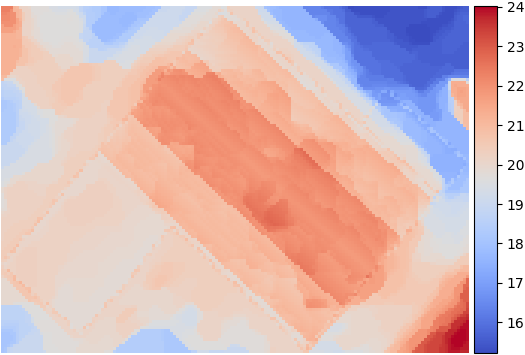
\includegraphics[width=3cm]{images/features/height/dsm-292034}};
        \path (dsm_1.south) node[anchor=north] (dsm_2) {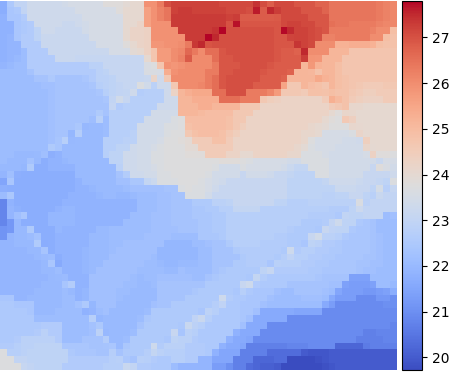
\includegraphics[width=3cm]{images/features/height/dsm-61215}};
        \path (dsm_2.south) node[anchor=north, text width=3cm] (dsm_legend) {\subcaption{\glspl{acr::dsm} \label{subfig::dsm}}};

        \path (dsm_1.east) node[anchor=west] (minus_1) {\Large --};
        \path (dsm_2.east) node[anchor=west] (minus_2) {\Large --};

		\path (minus_1.east) node[anchor=west] (model_1) {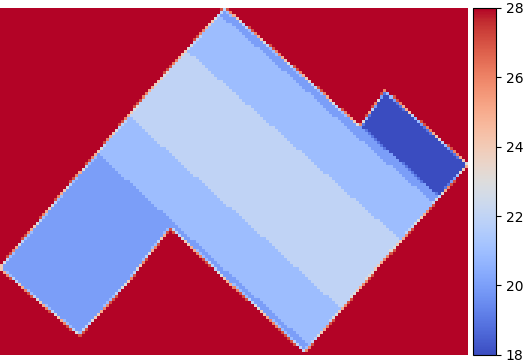
\includegraphics[width=3cm]{images/features/height/heightmap-292034}};
        \path (model_1.south) node[anchor=north] (model_2) {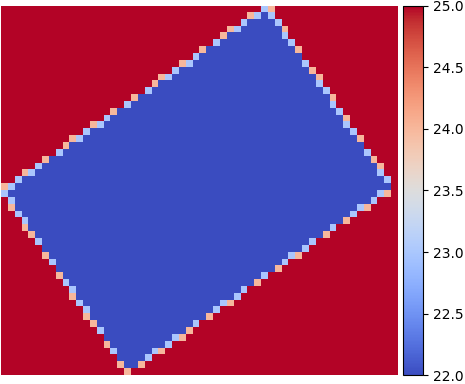
\includegraphics[width=3cm]{images/features/height/heightmap-61215}};
        \path (model_2.south) node[anchor=north, text width=3cm] (model_legend) {\subcaption{Model heights \label{subfig::height_map}}};

        \path (model_1.east) node[anchor=west] (equals_1) {\Large =};
        \path (model_2.east) node[anchor=west] (equals_2) {\Large =};

        \path (equals_1.east) node[anchor=west] (residual_1) {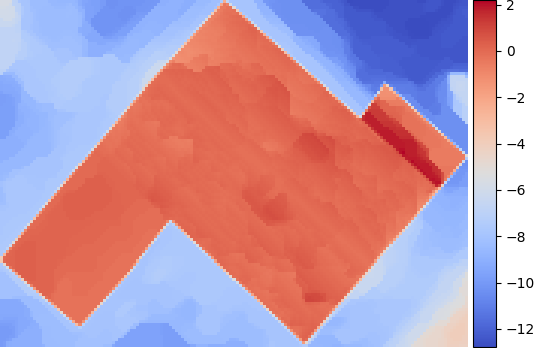
\includegraphics[width=3cm]{images/features/height/residual-292034}};
        \path (residual_1.south) node[anchor=north] (residual_2) {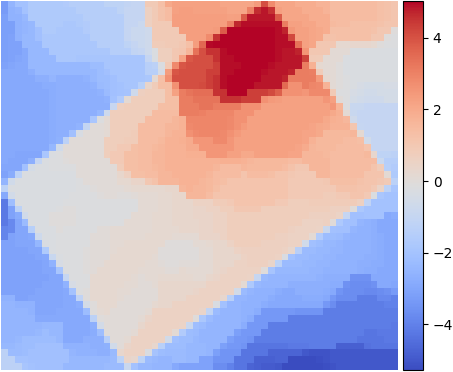
\includegraphics[width=3cm]{images/features/height/residual-61215}};
        \path (residual_2.south) node[anchor=north, text width=3cm] (residual_legend) {\subcaption{Residuals \label{subfig::residuals}}};

        \path (residual_1.east) + (0, .2) node[anchor=west] (top_dash_mapsto_1) {};
        \path (residual_1.east) + (0, -.2) node[anchor=west] (down_dash_mapsto_1) {};
        \draw (down_dash_mapsto_1) -- (top_dash_mapsto_1);
        \path (residual_2.east) + (0, .2) node[anchor=west] (top_dash_mapsto_2) {};
        \path (residual_2.east) + (0, -.2) node[anchor=west] (down_dash_mapsto_2) {};
        \draw (down_dash_mapsto_2) -- (top_dash_mapsto_2);

        \path (residual_1.east) + (.75, 0) node[anchor=west] (end_mapsto_1) {};
        \path (end_mapsto_1 |- residual_2) node[anchor=west] (end_mapsto_2) {};
        \draw[->] (top_dash_mapsto_1 |- residual_1) -- (end_mapsto_1) node[above, midway] {\scriptsize \(\chi\)};
        \draw[->] (top_dash_mapsto_2 |- residual_2) -- (end_mapsto_2) node[above, midway] {\scriptsize \(\chi\)};

        \path (end_mapsto_1.east) + (0, -1) node[anchor=west] (hist_1) {};
        \path (end_mapsto_2) + (0, -1) node[anchor=west] (hist_2) {};
        \path (hist_1 |- dsm_legend) + (1.25, 0) node[text width=3cm] (hist_legend) {\subcaption{Histogram \label{subfig::histogram}}};
        \begin{axis}[
            at={(hist_1)},
            width=4cm,
            area style,
            ymin=0,
            xmin=-14,
            xmax=14,
            yticklabels={,,}
        ]
            \addplot+[ybar interval,mark=no] plot coordinates {
                (-15, 0) 
                (-14, 0)
                (-13, 876)
                (-12, 366)
                (-11, 593)
                (-10, 675)
                (-9, 2231)
                (-8, 3623)
                (-7, 546)
                (-6, 159)
                (-5, 182)
                (-4, 70)
                (-3, 54)
                (-2, 123)
                (-1, 3815)
                (0, 4291)
                (1, 211)
                (2, 10)
                (3, 0)
                (4, 0)
                (5, 0)
                (6, 0)
                (7, 0)
                (8, 0)
            };
        \end{axis}
        \begin{axis}[
            at={(hist_2)},
            width=4cm,
            area style,
            ymin=0,
            xmin=-14,
            xmax=14,
            yticklabels={,,}
        ]
            \addplot+[ybar interval,mark=no] plot coordinates {
                (-15, 0)
                (-14, 0)
                (-13, 0)
                (-12, 0)
                (-11, 0)
                (-10, 0)
                (-9, 0)
                (-8, 0)
                (-7, 0)
                (-6, 17)
                (-5, 177)
                (-4, 143)
                (-3, 664)
                (-2, 219)
                (-1, 372)
                (0, 696)
                (1, 384)
                (2, 252)
                (3, 46)
                (4, 105)
                (5, 57)
                (6, 0)
                (7, 0)
                (8, 0)
            };
        \end{axis}
	\end{tikzpicture}
\end{document}
